\documentclass[11pt, headsepline]{article}

\usepackage[top=1in, bottom=1in, left=1in, right=1in]{geometry}
\usepackage{parskip}
\usepackage[colorlinks=true,linkcolor=blue,citecolor=blue,urlcolor=blue]{hyperref}
\usepackage{booktabs, cellspace, hhline, multirow, nicematrix}
\usepackage{float}
\usepackage{enumitem}
\usepackage{natbib}

\usepackage[usenames, dvipsnames]{xcolor}
\definecolor{sharpgreen}{rgb}{0.1, 0.55, 0.1}
\newcommand{\blue}[1]{\textcolor{blue}{#1}}
\newcommand{\red}[1]{\textcolor{red}{#1}}
\newcommand{\green}[1]{\textcolor{sharpgreen}{#1}}

\def\labelitemi{--}

\begin{document}

\section*{\centering \LARGE \normalfont Questionnaire}

\section*{Consent/screening}

\begin{enumerate}
    \item Thank you for your interest! We are a team of researchers from the University of Southern California conducting a study on economic preferences in the U.S. 
    The survey consists of multiple-choice and short-answer questions and will take approximately 15 minutes to complete.
    To participate, you must be a U.S. resident aged 18 or older. Do you confirm that you meet these criteria and would like to participate?

    Participation is voluntary, and you may exit the survey at any time. Your responses will be anonymous---no personally identifiable information will be retained, and you will not be personally identified in any findings. If you have any questions about the study, please contact us at nccarlso@usc.edu.

    \textit{Yes, I would like to participate and confirm that I am a U.S. resident aged 18 or older.; No, I do not wish to participate or do not meet the eligibility criteria.}
\end{enumerate}

\section*{Bot check}

\begin{enumerate}[resume]

    \item Please write the word “cactus” in the signature box below to confirm you are a human participant. This helps us ensure data quality. This is not a legal signature and will only be used for quality checks.

    [alternatively, ``banjo'']

    \textit{[signature box]}

\end{enumerate}

\section*{Age}

\begin{enumerate}[resume]

    \item What is your age?

    \textit{[text box]}

\end{enumerate}

\section*{Redistributive preferences}

\begin{enumerate}[resume]
    
    \item Should the government concern itself with reducing income differences between rich and poor people?

    \textit{The government should concern itself with this.; The government should not concern itself with this.}

    \green{GSS: ``Some people think that the government in Washington ought to reduce the income differences between the rich and the poor, perhaps by raising the taxes of wealthy families or by giving income assistance to the poor. Others think that the government should not concern itself with reducing this income difference between the rich and the poor. What score between 1 and 7 comes closest to the way you feel? \textit{The government should not concern itself with reducing income differences; The government should  concern itself with reducing income differences}''}

    \green{\cite{alesina2018intergenerational}: ``Some people think that the government (at the local, state, or federal level) should not care about income differences between rich and poor people. Others think that the government should do everything in its power to reduce income inequality. Rate on a scale of 1 to 7 on how you feel about this issue, with 1 being the government should not concern itself with income inequality and 7 being the government should do everything in its power to reduce income inequality.''}

    \green{ANES: ``Please say to what extent you agree or disagree with the following statement: The government should take measures to reduce differences in income levels.''}

    \blue{WVS waves 2-7: ``How would you place your views on this scale? \textit{(1) Incomes should be made more equal; (10) There should be greater incentives for individual effort}''}

    \blue{WVS waves 5-7: ``Please tell me for each of the following things how essential you think it is as a characteristic of democracy. \textit{Governments tax the rich and subsidize the poor.; The state makes people’s incomes equal.}''}

    \blue{GSS: ``To what extent do you agree or disagree with the following statements? \textit{Differences in income in America are too large.''}}

    \blue{GSS: ``From the following list, who do you think should have the greatest responsibility for reducing differences in income between people with high incomes and people with low incomes?''}

    \blue{GSS: ``Do you think people with high incomes should pay a larger share of their income in taxes than those with low incomes, the same share, or a smaller share?''}

    \blue{ANES: ``Favor/oppose government trying to reduce income inequality.''}

    \blue{\cite{stantcheva2021understanding}: ``Do you think that a progressive federal income tax system, in which people with higher incomes pay a higher share of income in taxes than people with lower incomes is an important tool to reduce inequality?''}
    
    \item Should the federal income tax be more progressive than it is now (redistributing more income from the rich to the poor)?

    [Randomly shown to half of the participants at the end of the survey, before the Demographics section.]

    \textit{Much more progressive (lower earners should pay a lot less than they do now and higher earners should pay a lot much more than they do now); Somewhat more progressive; No change; Somewhat less progressive; Much less progressive (everyone should be taxed at about the same rate)}

    \blue{GSS: ``Generally, how would you describe taxes in America today for those with high incomes? Taxes are...''}

    \blue{\cite{kuziemko2015elastic}: ``As you may know, there have been proposals recently to decrease the federal deficit by raising income taxes on millionaires. Do you think income taxes on millionaires should be increased, stay the same or decreased?''}

    \blue{\cite{kuziemko2015elastic}: Choose the tax rate on the top 1\%, next 9\%, next 40\% and bottom 50\%.}

    \blue{\cite{stantcheva2021understanding}: For these different groups, please tell me if you think that they are paying their fair share in federal taxes, paying too much, or paying too little? \textit{High income households; Middle-class households}''}

    \item How have your views about redistribution of income (from the rich to the poor) changed over time? 

    \textit{I now support redistribution much more than in the past; I now support redistribution slightly more than in the past; No change; I now support redistribution slightly less than in the past; I now support redistribution much less than in the past; Other: [text box]}

    \item Why did your views on redistribution improve? 
    
    [Only displayed if the respondent answered that they now support redistribution ``slightly more'' or ``much more.'']

    \textit{Taxes affect me less now; I think the policy is better for the economy now; I think the policy is more fair now; Other: [text box]}

    \item Why did your views on redistribution worsen? 
    
    [Only displayed if the respondent answered that they now support redistribution ``slightly less'' or ``much less.'']

    \textit{Taxes affect me more now; I think the policy is worse for the economy now; I think the policy is less fair now; Other: [text box]}
    
\end{enumerate}


\section*{Tax proposal (randomized)}

\begin{enumerate}[resume]
    \item Imagine the government is considering reducing federal income taxes for lower earners and raising federal income taxes for higher earners. There will be no change in total government spending, because the increased tax payments by the higher earners offset the reduced tax payments by the lower earners. 
    
    The proposed policy is pictured in gray in the figure below. The percentages shown are effective personal income tax rates, which represent what the average person pays after deductions, exemptions and credits. The policy only involves federal income taxes, so the percentages shown in the figure do not include taxes for medicare and social security, or state/local taxes.

    [Participants will be randomly shown one of the following proposals.]

    \underline{Poor benefit}
    \begin{figure}[H]
        \centering
        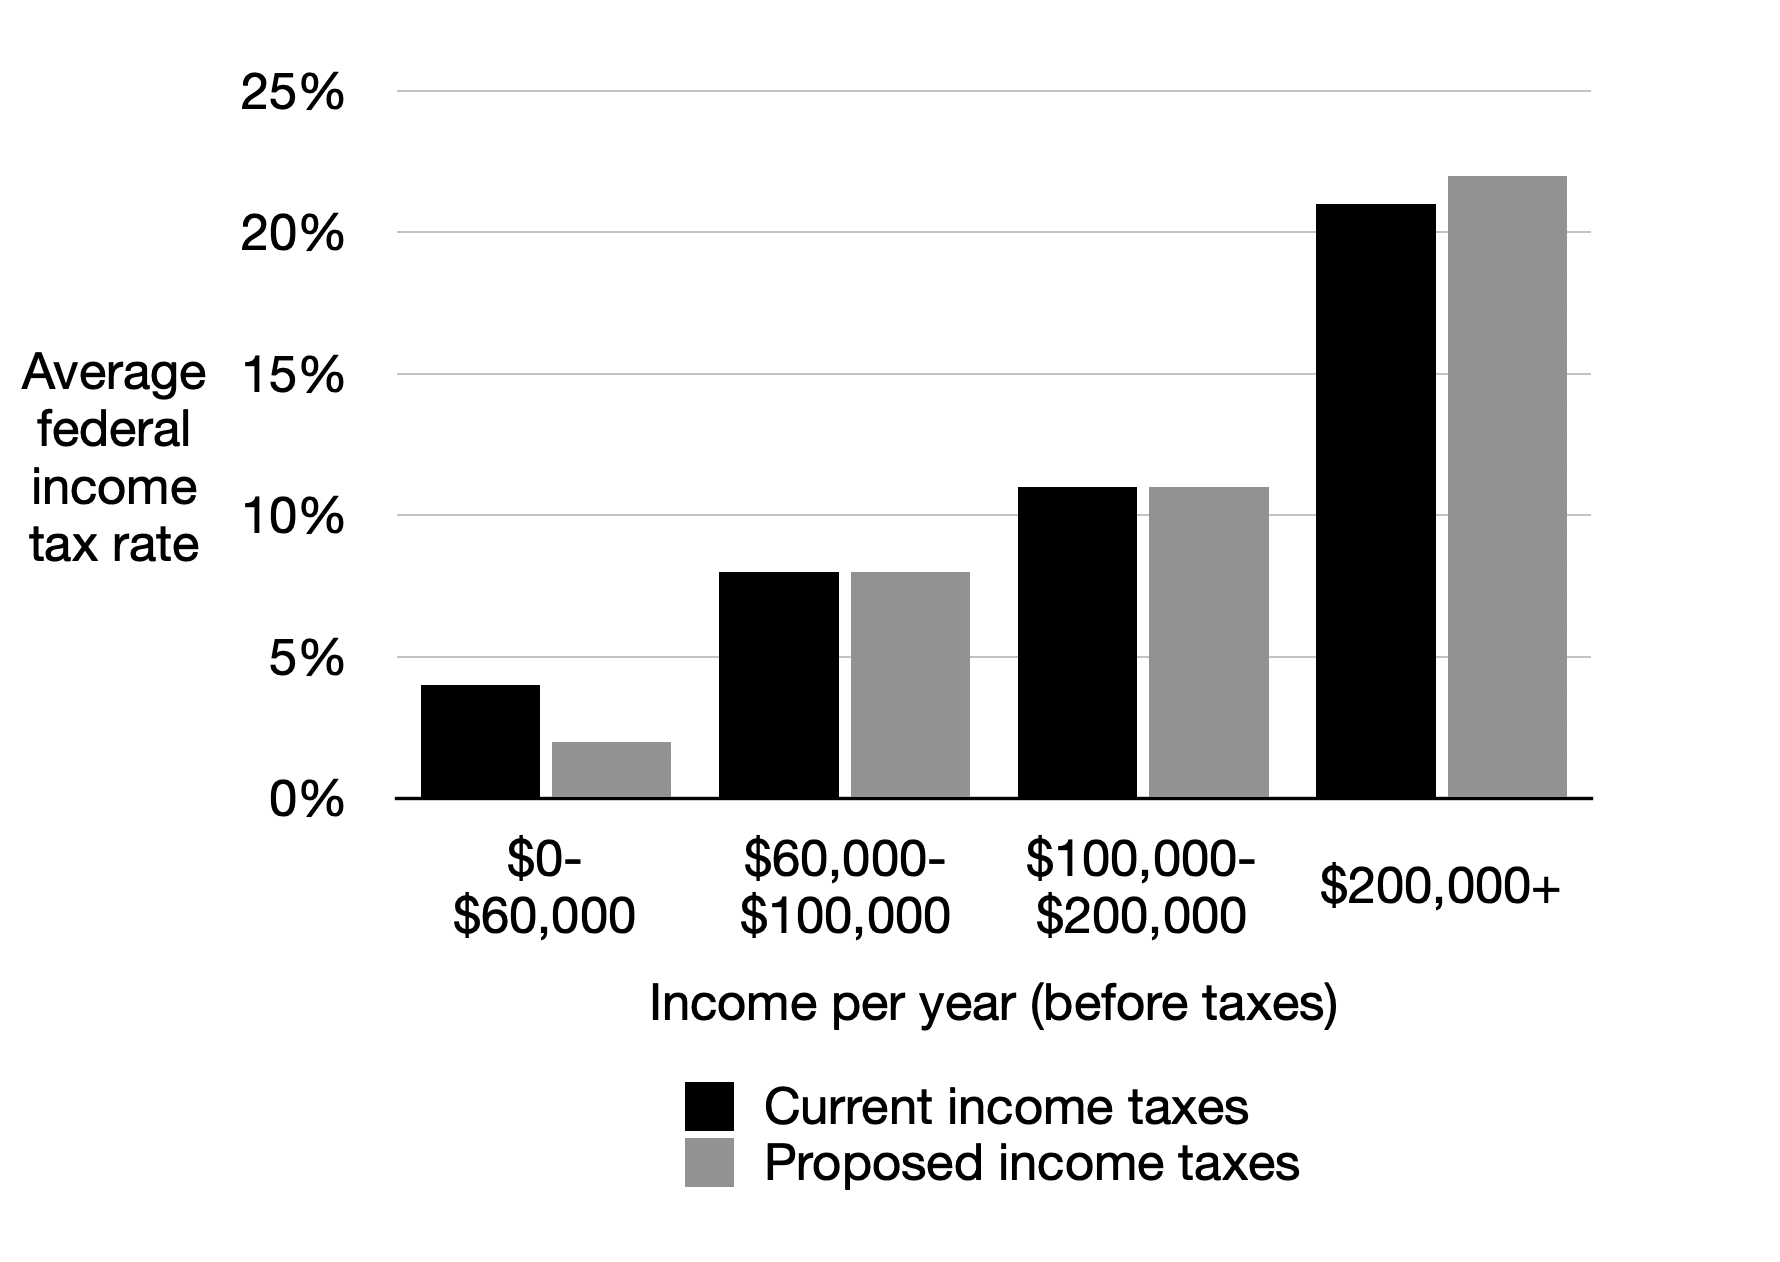
\includegraphics[width=0.7\linewidth]{images/poor.png}
        \label{fig:poor-benefit}
    \end{figure}
    \underline{Middle benefits}
    \begin{figure}[H]
        \centering
        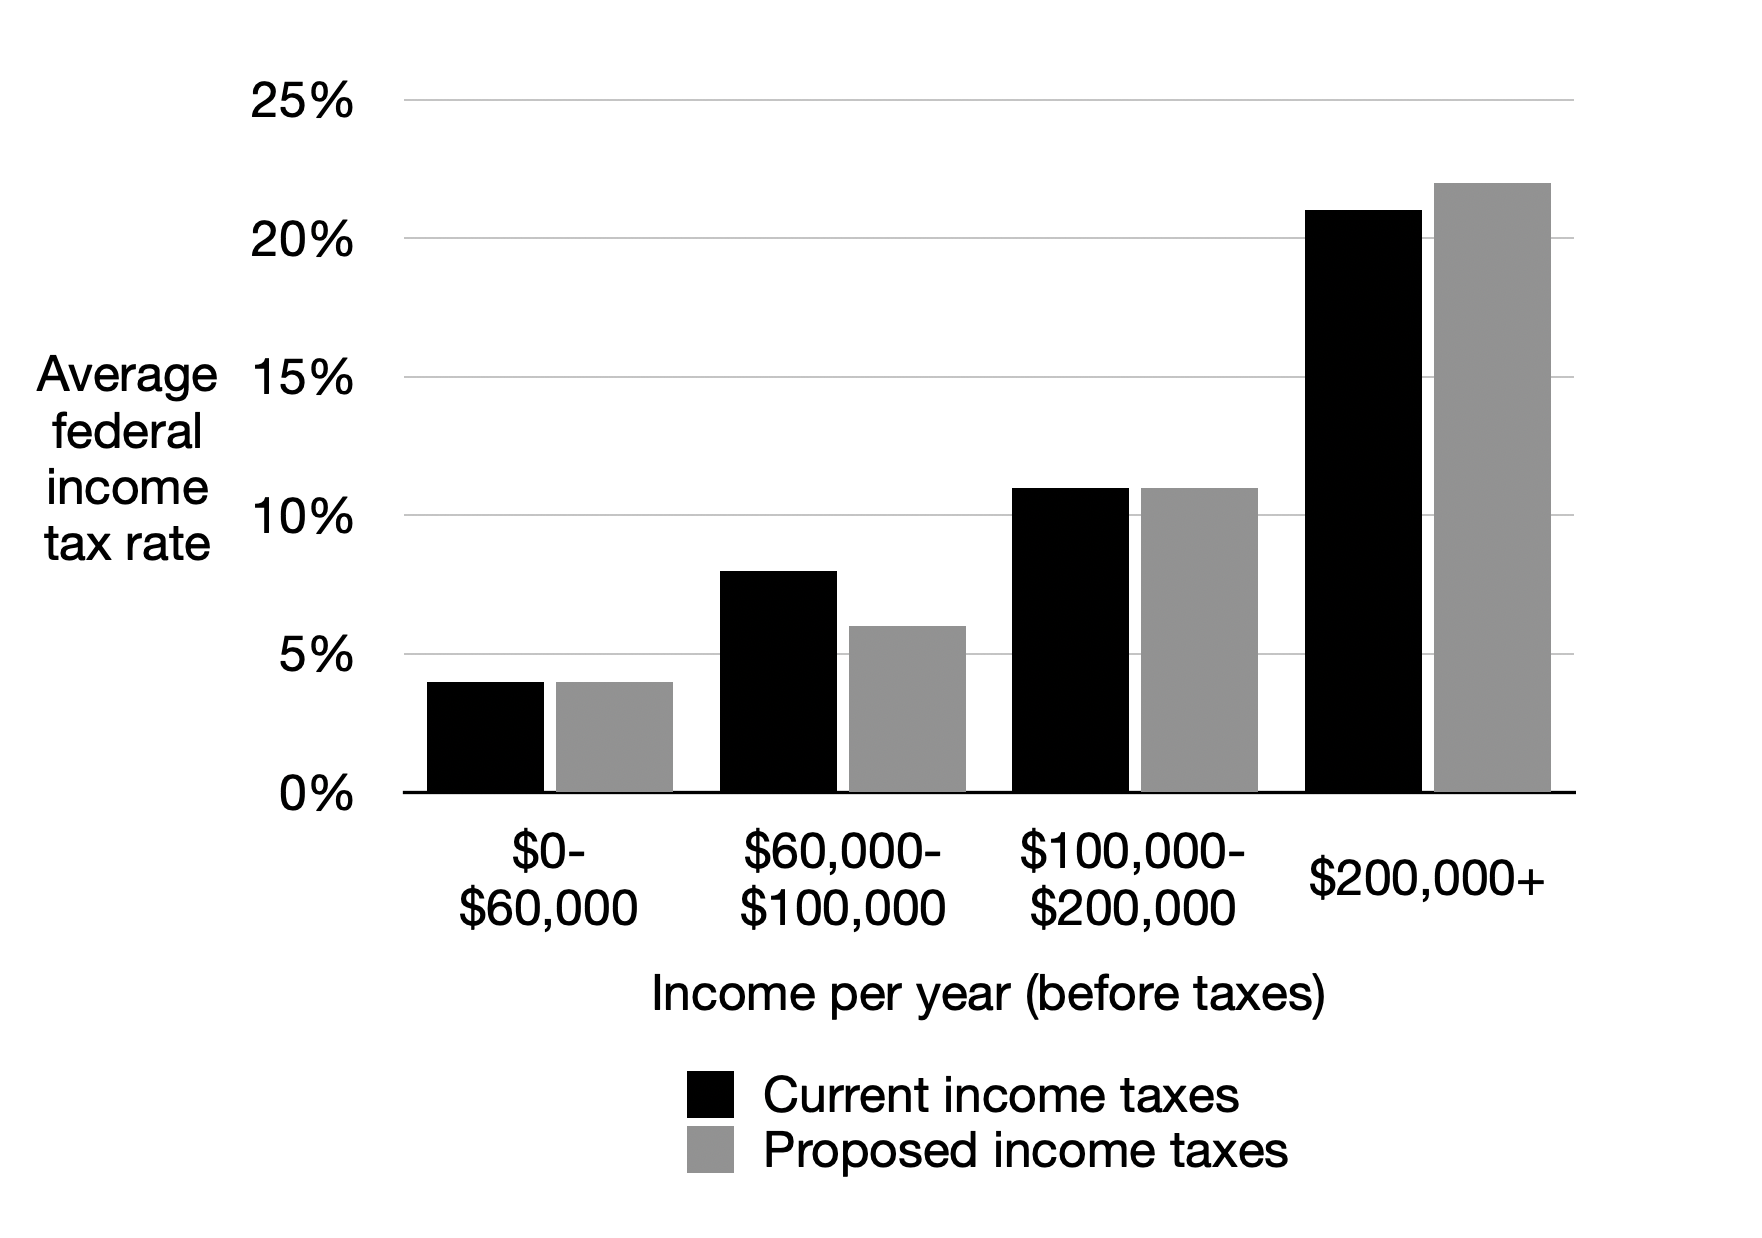
\includegraphics[width=0.7\linewidth]{images/middle.png}
        \label{fig:middle-benefit}
    \end{figure}
    \underline{Poor and middle both benefit}
    \begin{figure}[H]
        \centering
        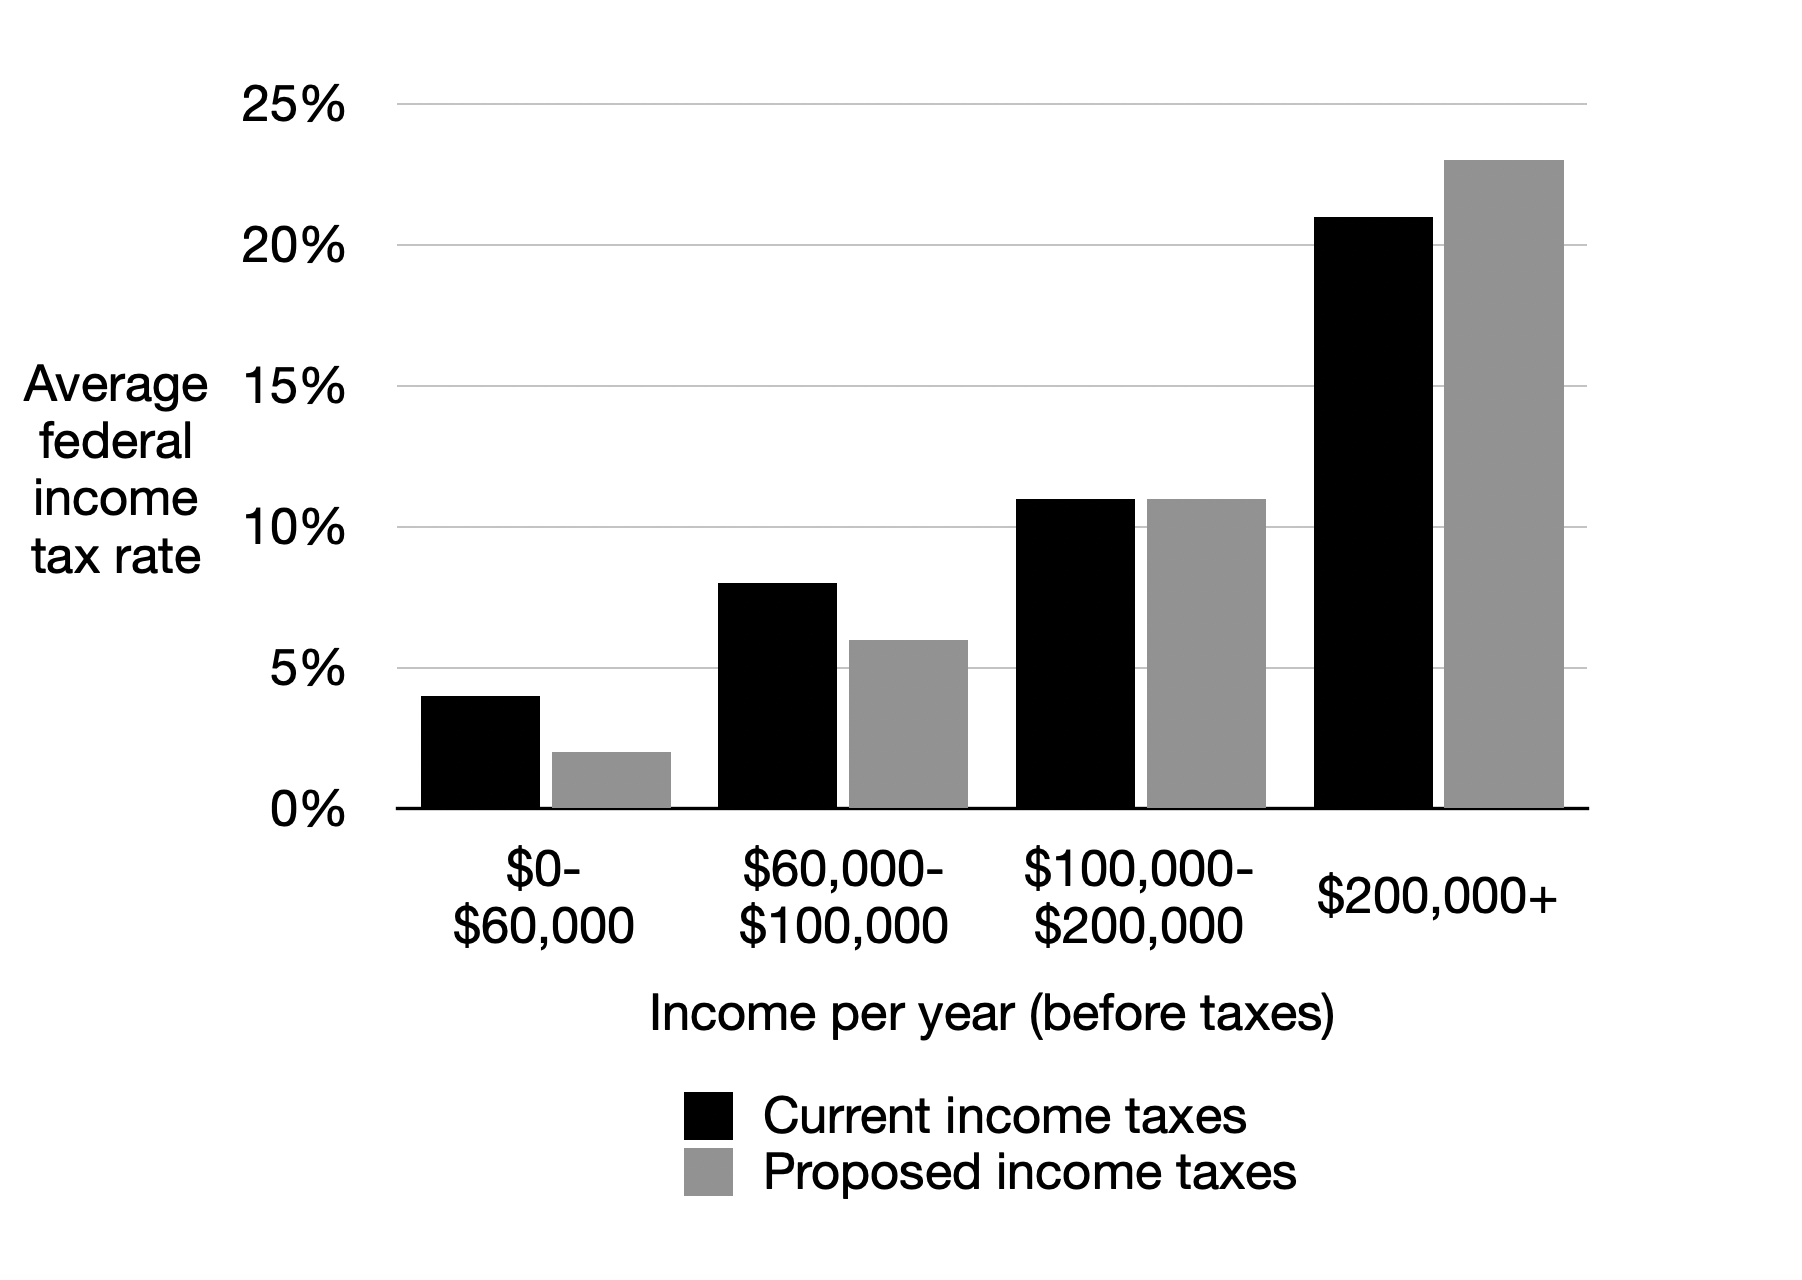
\includegraphics[width=0.7\linewidth]{images/both.png}
        \label{fig:both-benefit}
    \end{figure}

    Would you support or reject the proposed change?

    \textit{Support strongly; Support moderately; Support slightly; Indifferent; Reject slightly; Reject moderately; Reject strongly}
    
\end{enumerate}

\section*{Beliefs about incentive effects}

\blue{GSS: ``To what extent do you agree or disagree with the following statement? \textit{Large differences in income are necessary for America’s prosperity.}''}

\begin{enumerate}[resume]
    \item If taxes on high incomes are increased and taxes on low incomes are decreased, people will not work as hard in their jobs.

    \textit{Agree strongly; Agree somewhat; Neutral; Disagree somewhat; Disagree strongly; Unsure}

    \blue{\cite{stantcheva2021understanding}: ``If the federal personal income tax rate were to increase for the richest people in the economy [middle class], to what extent would it encourage them towards the following behaviors? \textit{Work less}''}

    \item A large income gap is needed to motivate entrepreneurs to start businesses and innovate.

    \textit{Agree strongly; Agree somewhat; Neutral; Disagree somewhat; Disagree strongly; Unsure}

     \blue{\cite{stantcheva2021understanding}: ``If the federal personal income tax rate were to increase for the richest people in the economy [middle class], to what extent would it encourage them towards the following behaviors? \textit{Be less entrepreneurial and create fewer businesses}''}
    
\end{enumerate}

\section*{Alternative policies}

\green{\cite{kuziemko2015elastic}: ``Which of the tools below do you consider the best to address inequality in the United States? Please drag and drop the items to the box on the right and rank them in your preferred order. Your preferred method for addressing inequality should be at the top, your least preferred one at the bottom. \textit{Education Policies, Private Charity, Progressive Taxes, Government Transfers (e.g., food stamps, Medicaid,..), Government regulation (e.g., min wage, caps on top compensation,...)}}

\begin{enumerate}[resume]
    \item To support lower-income and middle-income Americans, the government should focus on improving education quality and access.

    \textit{Agree strongly; Agree somewhat; Indifferent; Disagree somewhat; Disagree strongly; Unsure}

    \blue{GSS: ``Are we spending too much, too little, or the right amount on: Improving the nation's education system''}

    \blue{\cite{stantcheva2021understanding}: `` Take the following government services. For each of them, say if would you like it to receive increased funding (even if that means more taxes or reduced spending in other areas), decreased spending (in order to reduce taxes or increase spending elsewhere) or would you like for its funding to be left unchanged? Better schools for children from low-income families''}

    \blue{\cite{alesina2023immigration}: ``Would you say that you strongly favor, favor, neither favor nor oppose, oppose or strongly oppose spending more money on schools in poor neighborhoods?''}

    \item To support lower-income and middle-income Americans, the government should focus on protecting domestic jobs from international competition, for example, through tariffs.

    \textit{Agree strongly; Agree somewhat; Indifferent; Disagree somewhat; Disagree strongly; Unsure}

    \blue{GSS: ``To what extent do you agree or disagree with the following statements? Workers need strong trade unions to protect their interests.''}

    \blue{GSS: ``The government should support declining industries to protect jobs, even if it might require a tax increase to pay for it.''}

    \blue{ANES: ``Do you favor, oppose, or neither favor nor oppose the U.S. making free trade agreements with other countries?''}

    \blue{ANES: ``Has international trade increased, decreased, or neither increased nor decreased the number of jobs available in the United States?''}

    \item To support lower-income and middle-income Americans, the government should focus on cutting taxes by reducing government services.

    \textit{Agree strongly; Agree somewhat; Indifferent; Disagree somewhat; Disagree strongly; Unsure}

    \blue{ANES: ``Some people think the government should provide fewer services even in areas such as health and education in order to reduce spending. Suppose these people are at one end of a scale, at point 1. Other people feel it is important for the government to provide many more services even if it means an increase in spending. Suppose these people are at the other end, at point 7.''}

    \blue{\cite{stantcheva2021understanding}: ``What do you think would ultimately do more to reduce the income differences between poor and rich families? \textit{Lowering taxes on wealthy people/women and corporations to encourage more investment in economic growth.; Raising taxes on wealthy people/women and corporations to expand programs for the poor.}''}

    \item To support lower-income and middle-income Americans, the government should introduce publicly funded universal health insurance for all Americans (with the possibility to still purchase extra private insurance).

    \textit{Agree strongly; Agree somewhat; Indifferent; Disagree somewhat; Disagree strongly; Unsure}

    \blue{ANES: ``How well do you think that our political system guarantees adequate healthcare for all citizens?''}

    \blue{GSS: ``Are we spending too much, too little, or the right amount on: Improving and protecting the nation's health''}

    \item To support lower-income and middle-income Americans, the government should introduce a federal wealth tax on high-wealth individuals.

    \textit{Agree strongly; Agree somewhat; Indifferent; Disagree somewhat; Disagree strongly; Unsure}

    \blue{\cite{stantcheva2021understanding}: ``Do you think the federal estate tax should be increased, left at the current level, or lowered?''}
    
\end{enumerate}

\section*{Zero-sum beliefs}

\begin{enumerate}[resume]

    \item People usually get rich at the expense of others rather than by creating value for others.

    \textit{Agree strongly; Agree somewhat; Neither agree nor disagree; Disagree somewhat; Disagree strongly; Unsure}

    \green{WVS waves 2-3 and 5-7: ``How would you rate your views on this scale? \textit{(1) People can only get rich at the expense of others; (10) Wealth can grow so there’s enough for everyone}''}

    \item In recent decades, large gains in CEO and executive salaries have been at the expense of the salaries of average workers.

    \textit{Agree strongly; Agree somewhat; Neither agree nor disagree; Disagree somewhat; Disagree strongly; Unsure}

    \red{Should be something similar out there.}

    \item In recent decades, women’s wage gains have been at the expense of men’s wages.

    \textit{Agree strongly; Agree somewhat; Neither agree nor disagree; Disagree somewhat; Disagree strongly; Unsure}

    \item Diversity, equity, and inclusion (DEI) initiatives create opportunities for some at the expense of others.

    \textit{Agree strongly; Agree somewhat; Neither agree nor disagree; Disagree somewhat; Disagree strongly; Unsure}
    
\end{enumerate}

\section*{Current state of mobility and personal mobility}

\begin{enumerate}[resume]

    \item Consider a child coming from the poorest 20\% of families in the U.S. today. They are very determined and work hard in school, and later in life, they will work hard at their career. What do you believe is the chance that they make it into the richest 20\% of families/individuals when they are older?

    \green{\cite{alesina2018intergenerational}: ``For the following questions, we focus on 500 families that represent the U.S. population. We divide them into five groups on the basis of their income, with each group containing 100 families. These groups are: the poorest 100 families, the second poorest 100 families, the middle 100 families, the second richest 100 families, and the richest 100 families. [Consider 100 children coming from the poorest 100 families. These children are very determined and put in hard work both at school and, later in life, when finding a job and doing that job.] Do you think the chances that a child from the poorest 100 families [one of these hardworking children] will grow up to be among the second richest 100 families are: \textit{Close to zero; Low; Fairly low; Fairly high; High}''}

    \textit{Almost guaranteed (80-100\%); Likely (60-80\%); Even chance (40-60\%); Unlikely (20-40\%); Almost no chance (0-20\%); Unsure}

    \item What do you believe is the chance that they make it into the richest 50\% of families/individuals when they are older?

    \textit{Almost guaranteed (80-100\%); Likely (60-80\%); Even chance (40-60\%); Unlikely (20-40\%); Almost no chance (0-20\%); Unsure}

    \item Is it harder or easier to move up in the U.S. now than when your parents were growing up (in terms of income/wealth)?

    \textit{Much harder now; Somewhat harder now; No change; Somewhat easier now; Much easier now; Unsure}

    \red{Should be something similar out there.}

    \item Thinking about your past achievements, do you believe that your hard work in life has paid off or not?

    \textit{It has paid off a lot; It has paid off somewhat; It has not paid off much; Unsure}

    \blue{GSS: ``Some people say that people get ahead by their own hard work; others say that lucky breaks or help from other people are more important. Which do you think is most important?''}

    \blue{GSS: ``For each of these, please tell me how important it is for getting ahead in life: \textit{How important is hard work?}}

    \blue{GSS: ``Some people say that people get ahead by their own hard work; others say that lucky breaks or help from other people are more important. Which do you think is most important?''}

    \item Thinking about your future achievements, do you believe that your hard work in life will pay off or not?

    \textit{It will pay off a lot; It will pay off somewhat; It will not pay off much; Unsure}

    \item Do you believe your education will pay off in terms of economic opportunity?

    \textit{It will pay off a lot; It will pay off somewhat; It will not pay off much; Unsure}

    \red{Should be something similar out there.}
    
\end{enumerate}

\section*{Family mobility and relative income}

\begin{enumerate}[resume]

    \item When your mother (or first caretaker) was growing up, how did her (or their) family income compare to other American families?

    \textit{Far below average; Below average; Average; Above average; Far above average; Unsure / Not applicable}

    \blue{WVS wave 7: ``Comparing your standard of living with your parents’ standard of living when they were about your age, would you say that you are better off, worse off or about the same?''}

    \blue{GSS: ``Compared to your parents when they were the age you are now, do you think your own standard of living now is much better, somewhat better, about the same, somewhat worse, or much worse than theirs was?''}

    \item When your father (or second caretaker) was growing up, how did his (or their) family income compare to other American families?

    \textit{Far below average; Below average; Average; Above average; Far above average}

    \item When you were growing up, how did your family income compare to other American families?

    \textit{Far below average; Below average; Average; Above average; Far above average}

    \green{\cite{alesina2018intergenerational}: ``When you were growing up, compared with American families back then, would you say your family income was: \textit{Far below average; Below average; Average; Above average; Far above average}''}

    \item Right now, how does your personal income compare with other Americans your age?

    \textit{Far below average; Below average; Average; Above average; Far above average}

    \green{\cite{alesina2018intergenerational}: ``Right now, compared with American families, would you say your own household income is: \textit{Far below average; Below average; Average; Above average; Far above average}''}

    \blue{\cite{hvidberg2023social}:}
    
\end{enumerate}

\section*{Income uncertainty}

\begin{enumerate}[resume]

    \item In the following questions, we will define personal income as income you earned yourself in a given year, and household income as the total income earned by yourself and any spouse, partner, or children under your care old enough to work. Income includes earnings from wages, self-employment, investment returns, pensions and retirement withdrawals.
    
    Are you the only person in your household or the only person earning income in your household?

    \textit{Yes; No, someone else also earns income}

    \item In 10 years, do you expect that more than one person in your household will be earning income? 

    \textit{Yes, more than one person; No, just myself}

    \item What was your total personal income (before taxes) last year (2024)?

    It is fine to approximate. Please enter a number such as 50,000 or 50000, but not \$50,000.

    \textit{[text box]}

    \item What do you expect your annual personal income (before taxes) to be 10 years from now?

    Please ignore inflation and answer using the value of a dollar today.

    \textit{[text box]}

    \blue{NY Fed SCE: ``Over the next 12 months, what do you expect will happen to the total income of all members of your household (including you), from all sources before taxes and deductions? \textit{Increase; Decrease} By about what percent do you expect your total household income to [increase/decrease]? Please give your best guess.''}

    \red{Not much for longer time frames. Potentially something in RAND ALP.}

    \item How certain are you that your personal income will be close to this number?

    \textit{Very certain; Somewhat certain; Not very certain}

     \item Thinking ahead 10 years, what is the highest your annual personal income (before taxes) might be under good—but still realistic—circumstances?

    \textit{[text box]}

    \item Thinking ahead 10 years, what is the lowest your annual personal income (before taxes) might be under bad—but still realistic—circumstances?

    \textit{[text box]}

    [The following questions in this section appear according to the responses at the beginning.]

    \item What was your total household income (before taxes) last year (2024)?

    \textit{[text box]}

    \item What do you expect your annual household income (before taxes) to be 10 years from now? 

    \textit{[text box]}

    \item How certain are you that your household income will be close to this number?

    \textit{Very certain; Somewhat certain; Not very certain}

    \item Thinking ahead 10 years, what is the highest your annual household income (before taxes) might be under good—but still realistic—circumstances?

    \textit{[text box]}

    \item Thinking ahead 10 years, what is the lowest your annual household income (before taxes) might be under bad—but still realistic—circumstances?

    \textit{[text box]}
    
\end{enumerate}

\section*{Perceived future income needs}

\begin{enumerate}[resume]
    \item At least how much annual household income (before taxes) would you need to live comfortably now?

    \textit{[text box]}

    \red{Fed Board SCF, WVS, GSS, ANES have more general questions about financial situation/satisfaction.}

    [The following questions in this section appear only if the respondent is under 30 years old.]
    
    \item Is it more likely that you will or  will not have children to support in your 30s?

    \textit{Will have children; Will not have children}

    \item Assuming your answer to the previous question becomes true, how much annual household income (before taxes) will you need to live comfortably in your 30s?

    \textit{[text box]}

    \item Is it more likely that you will or will not have children to support in your 40s?

    \textit{Will have children; Will not have children}

    \item Assuming your answer to the previous question becomes true, how much annual household income (before taxes) will you need to live comfortably in your 40s?

    \textit{[text box]}
    
\end{enumerate}

\section*{Generosity and universalism}

\begin{enumerate}[resume]

    \item Imagine you unexpectedly receive \$100 as a gift. You have the option to keep all of it for yourself or give some of it to a complete stranger who is struggling to afford basic necessities. The money cannot be given to anyone else or donated elsewhere.

    How much of the \$100 would you choose to give to the stranger?

    \textit{[text box]}

    \red{A variant of the dictator game.}
    
    \green{\cite{enke2023moral}: ``...respondents made five decisions, in each of which they were asked to split hypothetical \$100 between (1) a randomly selected person who lives anywhere in the world and (2) a randomly selected person who lives anywhere in the world and is a member of the respondent’s social groups. Across the five questions, the social groups included the same language, same religious beliefs, same ethnic background, same values, and same occupation. The average amount of money sent to the randomly selected world citizen makes up the global universalism measure.''}

    \item Imagine again that you unexpectedly receive \$100 as a gift. You have the option to keep all of it for yourself or give some of it to a friend or family member. The money cannot be given to anyone else or donated elsewhere.

    How much of the \$100 would you choose to give to a friend or family member?

    \textit{[text box]}
    
\end{enumerate}

\section*{Time discounting}

\begin{enumerate}[resume]

    \item Would you prefer \$1,000 today or \$1,100 in 1 year?

    \green{\cite{falk2018global}: ``Suppose you were given the choice between receiving a payment today or a payment in 12 months. We will now present to you five situations. The payment today is the same in each of these situations. The payment in 12 months is different in every situation. For each of these situations we would like to know which one you would choose. Please assume there is no inflation, i.e., future prices are the same as today’s prices. Please consider the following: Would you rather receive amount x today or y in 12 months?''} 
    
    \red{Time-discounting literature.}

    \textit{\$1,000 today; \$1,100 in 1 year; Indifferent}

    \item Would you prefer \$1,000 today or \$1,500 in 1 year?

    \textit{\$1,000 today; \$1,500 in 1 year; Indifferent}

    \item Would you prefer \$1,000 today or \$2,000 in 1 year?

    \textit{\$1,000 today; \$2,000 in 1 year; Indifferent}

    \item Would you prefer \$1,000 today or \$1,100 in 5 years?

    \textit{\$1,000 today; \$1,100 in 5 years; Indifferent}

    \item Would you prefer \$1,000 today or \$1,500 in 5 years?

    \textit{\$1,000 today; \$1,500 in 5 years; Indifferent}

    \item Would you prefer \$1,000 today or \$2,000 in 5 years?

    \textit{\$1,000 today; \$2,000 in 5 years; Indifferent}

    \item I often prioritize my current needs and desires, even if it means delaying my long-term goals.

    \textit{Agree strongly; Agree somewhat; Indifferent; Disagree somewhat; Disagree strongly}

    \green{\cite{strathman1994consideration}: Consideration of Future Consequences (CFC) scale. Includes questions such as ``I only act to satisfy immediate concerns, figuring the future will take care of itself.''}

    \blue{\cite{falk2018global}: ``How willing are you to give up something that is beneficial for you today in order to benefit more from that in the future?''}
    
\end{enumerate}


\section*{Career plans and materialism}

\begin{enumerate}[resume]

    \item What do you value most in a job? Please rank top to bottom from most to least important by clicking or tapping on the choice tabs and dragging them up or down.

    \textit{Salary and benefits; Reasonable workload and/or flexible hours; Career growth and development; Meaningful and/or challenging work; Positive work environment and relationships}

    \green{WVS waves 3-5: ``Which one would you place first if you were looking for a job? \textit{A good income so that you do not have any worries about money; A safe job with no risk of closing down or unemployment; Working with people you like; Doing an important job which gives you a feeling of accomplishment''}}

    \blue{WVS waves 1-4: ``What is important in a job? \textit{Good pay; Not too much pressure; Good job security; A respected job; A job that is interesting; That you can achieve something}''}

    \item I would be satisfied with a modest income that covers basic needs—food, housing, clothing, healthcare, transportation—with a small amount left over for occasional extras.

    \textit{Agree strongly; Agree somewhat; Neutral; Disagree somewhat; Disagree strongly}

    \blue{GSS: ``If you were to get enough money to live as comfortably as you would like for the rest of your life, would you continue to work or would you stop working?''}

    \item Do you plan on starting a business at some point?

    \textit{Definitely / I have already started a business; Probably; Maybe; Probably not; Definitely not}

\end{enumerate}

\section*{Financial (in)security}

\begin{enumerate}[resume]

    \item How stable is your current primary source of income?

    \textit{Very stable; Somewhat stable; Neutral; Somewhat unstable; Very unstable}

    \blue{GSS: ``We are interested in how people are getting along financially these days. So far as you and your family are concerned, would you say that you are pretty well satisfied with your present financial situation, more or less satisfied, or not satisfied at all?''}

    \blue{GSS: ``During the last few years, has your financial situation been getting better, worse, or has it stayed the same?''}

    \blue{GSS: ``Thinking of your household's total income, including all the sources of income of all the members who contribute to it, how difficult or easy is it currently for your household to make ends meet?''}

    \item To what degree are you worried about losing your job or not finding a job?

    \textit{Very worried; Somewhat worried; Not very worried; Not worried at all}

    \green{WVS waves 6-7: ``To what degree are you worried about losing your job or not finding a job?''}

    \blue{NY Fed SCE: ``What do you think is the percent chance that you will lose your [main/current] job during the next 12 months?''}

    \blue{GSS: ``Thinking about the next 12 months, how likely do you think it is that you will lose your job or be laid off?''}

    \item If you were to lose your job in the next 12 months, how likely is it that you would find a job with similar or higher pay within 3 months?

    \textit{Almost certain (90-100\%); Likely (60-90\%); Even chance (40-60\%); Unlikely (10-40\%); Almost no chance (0-10\%)}

    \green{NY Fed SCE: ``Suppose you were to lose your job this month. What do you think is the percent chance that within the following 3 months, you will find a job that you will accept, considering the pay and type of work?''}

    \blue{GSS: ``About how easy would it be for you to find a job with another employer with approximately the same income and fringe benefits you now have?''}

    \item If you lost your source of income, how long could you maintain your current lifestyle using your financial safety net (savings and assets)?

    \textit{Less than 1 month; 1-3 months; 3-6 months; More than 6 months}

    \blue{WVS waves 3-7: Family savings during the past year.}

    \red{Fed Board SHED and SCF may ask about ability to come up with money to cover unexpected expenses}

\end{enumerate}

\section*{Existential uncertainty}

\begin{enumerate}[resume]

    \item What is the risk of losing your job to artificial intelligence (AI) in the next 10 years?

    \textit{I have already lost a job to AI; The risk is high; The risk is substantial; The risk is low; No risk}

    \item What is the risk that you have to relocate due to climate events in the next 10 years?

    \textit{I have already relocated due to climate events; The risk is high; The risk is substantial; The risk is low; No risk}

    \item What is the risk that you have to live without health insurance in the next 10 years?

    \textit{I already live without health insurance; The risk is high; The risk is substantial; The risk is low; No risk}

    \item What is the risk that you are unable to ever own a home?

    \textit{The risk is high; The risk is substantial; The risk is low; No risk; I have already owned or currently own a home}

\end{enumerate}

\section*{Demographics}

\blue{Most surveys include many of these questions.}

Thank you for making it this far! To conclude, we would like to ask you some demographic questions.

\begin{enumerate}[resume]

    \item What is your gender?

    \textit{Male; Female; Non-binary; Prefer not to say}

    \item Please indicate your marital status.

    \textit{Single; Married; Cohabitating; Other: [text box]}

    \item How many children have you had?

    \textit{I do not have children; 1; 2; 3; 4; 5 or more}

    \item How many children in total do you plan on having over your lifetime?

    \textit{0; 1; 2; 3; 4; 5 or more; Unsure}

    \item How would you describe your ethnicity and/or race?

    \textit{American Indian or Alaska Native; Asian or Asian American; Black or African American; Hispanic or Latino; Middle Eastern or North African; Native Hawaiian or Pacific Islander; 
    White or European American; Other: [text box]}

    \item Were you born in the United States?

    \textit{Yes; No}

    \item Were both of your parents born in the United States?

    \textit{Yes; No}

    \item In which state do you currently reside? (If you are in college or temporarily stationed with the military, please enter the location you spend the most time in.)

    \textit{[state dropdown]}

    \item What is your current 5-digit ZIP code? (If you are in college or temporarily stationed with the military, please enter the location you spend the most time in. You may skip if you are not sure.)

    \textit{[text box]}

    \item Would you consider your current location urban, suburban, or rural?

    \textit{Urban; Suburban; Rural}

    \item Which state do you consider your home state (birthplace or place you grew up)?

    \textit{[state dropdown]}

    \item What is the name of your home town or city (birthplace or place you grew up)?

    \textit{[text box]}

    \item Would you consider your home town or city urban, suburban, or rural?

    \textit{Urban; Suburban; Rural}

    \item Are you a student right now?

    \textit{Not a student; High school; 2-year college; 4-year college; Master’s degree (e.g., MA, MS, MBA); Research doctoral program (e.g., PhD, DSc); Professional doctoral program (e.g., JD, MD)}

    \item Which category best describes your highest level education?

    \textit{Eighth grade or less; Some high school; High school degree / GED; Some college; 2-year college degree; 4-year college degree; Master’s degree (e.g., MA, MS, MBA); Research doctorate (e.g., PhD, DSc); Professional doctorate (e.g., JD, MD)}

    \item What is the highest level of education you plan on obtaining?

    \textit{Eighth grade or less; Some high school; High school degree / GED; Some college; 2-year college degree; 4-year college degree; Master’s degree (e.g., MA, MS, MBA); Research doctorate (e.g., PhD, DSc); Professional doctorate (e.g., JD, MD)}

    \item Which category best describes your mother's (or first caregiver's) highest level of education?

    \textit{Eighth grade or less; Some high school; High school degree / GED; Some college; 2-year college degree; 4-year college degree; Master’s degree (e.g., MA, MS, MBA); Research doctorate (e.g., PhD, DSc); Professional doctorate (e.g., JD, MD)}

    \item Which category best describes your father's (or second caregiver's) highest level of education?

    \textit{Eighth grade or less; Some high school; High school degree / GED; Some college; 2-year college degree; 4-year college degree; Master’s degree (e.g., MA, MS, MBA); Research doctorate (e.g., PhD, DSc); Professional doctorate (e.g., JD, MD)}

    \item What is your current employment status?

    \textit{Full-time employee; Part-time employee; Self-employed or small business owner; Unemployed and looking for work; Student; Not in the labor force (for example: retired, or full-time parent)}

    \item On economic policy matters, where do you see yourself on the liberal/conservative spectrum?
    
    \textit{Liberal; Moderate; Conservative}

    \item On social policy matters, where do you see yourself on the liberal/conservative spectrum?
    
    \textit{Liberal; Moderate; Conservative}

    \item Who did you vote for in the 2024 U.S. presidential election?

    \textit{Kamala Harris; Donald Trump; Other; I did not vote}

    \item Who did you vote for in the 2020 U.S. presidential election?

    \textit{Joe Biden; Donald Trump; Other; I did not vote}

\end{enumerate}

\section*{Feedback}

\begin{enumerate}[resume]

    \item Do you feel that this survey was left- or right-wing biased or unbiased?

    \textit{Left-wing biased; Right-wing biased; Unbiased}

    \item Let us know if you have any feedback—we're especially interested in whether any questions were confusing or if the survey length felt appropriate. Otherwise, we thank you for participating in the project!

    \textit{[text box]}
    
\end{enumerate}

\newpage
\bibliographystyle{apalike}
\bibliography{refs}

\end{document}